% Options for packages loaded elsewhere
\PassOptionsToPackage{unicode}{hyperref}
\PassOptionsToPackage{hyphens}{url}
%
\documentclass[
]{article}
\usepackage{amsmath,amssymb}
\usepackage{iftex}
\ifPDFTeX
  \usepackage[T1]{fontenc}
  \usepackage[utf8]{inputenc}
  \usepackage{textcomp} % provide euro and other symbols
\else % if luatex or xetex
  \usepackage{unicode-math} % this also loads fontspec
  \defaultfontfeatures{Scale=MatchLowercase}
  \defaultfontfeatures[\rmfamily]{Ligatures=TeX,Scale=1}
\fi
\usepackage{lmodern}
\ifPDFTeX\else
  % xetex/luatex font selection
\fi
% Use upquote if available, for straight quotes in verbatim environments
\IfFileExists{upquote.sty}{\usepackage{upquote}}{}
\IfFileExists{microtype.sty}{% use microtype if available
  \usepackage[]{microtype}
  \UseMicrotypeSet[protrusion]{basicmath} % disable protrusion for tt fonts
}{}
\makeatletter
\@ifundefined{KOMAClassName}{% if non-KOMA class
  \IfFileExists{parskip.sty}{%
    \usepackage{parskip}
  }{% else
    \setlength{\parindent}{0pt}
    \setlength{\parskip}{6pt plus 2pt minus 1pt}}
}{% if KOMA class
  \KOMAoptions{parskip=half}}
\makeatother
\usepackage{xcolor}
\usepackage[margin=1in]{geometry}
\usepackage{graphicx}
\makeatletter
\def\maxwidth{\ifdim\Gin@nat@width>\linewidth\linewidth\else\Gin@nat@width\fi}
\def\maxheight{\ifdim\Gin@nat@height>\textheight\textheight\else\Gin@nat@height\fi}
\makeatother
% Scale images if necessary, so that they will not overflow the page
% margins by default, and it is still possible to overwrite the defaults
% using explicit options in \includegraphics[width, height, ...]{}
\setkeys{Gin}{width=\maxwidth,height=\maxheight,keepaspectratio}
% Set default figure placement to htbp
\makeatletter
\def\fps@figure{htbp}
\makeatother
\setlength{\emergencystretch}{3em} % prevent overfull lines
\providecommand{\tightlist}{%
  \setlength{\itemsep}{0pt}\setlength{\parskip}{0pt}}
\setcounter{secnumdepth}{-\maxdimen} % remove section numbering
\ifLuaTeX
  \usepackage{selnolig}  % disable illegal ligatures
\fi
\IfFileExists{bookmark.sty}{\usepackage{bookmark}}{\usepackage{hyperref}}
\IfFileExists{xurl.sty}{\usepackage{xurl}}{} % add URL line breaks if available
\urlstyle{same}
\hypersetup{
  pdftitle={Networks HW1},
  pdfauthor={izd3},
  hidelinks,
  pdfcreator={LaTeX via pandoc}}

\title{Networks HW1}
\author{izd3}
\date{2023-08-26}

\begin{document}
\maketitle

\textbf{1.)}A group of economists are studying the interactions between
10 banks. They drew the graph in Figure 1 to describe these interactions
with nodes representing the banks and edges between two nodes
representing the idea that these two banks interact with each other. So
for example, banks A and D interact, but banks A and B do not interact.
These ``interactions'' are meant to describe economic transactions
between the banks. These economists are interested in measuring how
important individual banks are purely as a function of their location in
this network. One way they are considering is to count the degree of
each bank. The degree of a node in an undirected graph such as Figure 1
is the number of edges attached to the node.

\textbf{A.)}For each node in Figure 1, what is it's degree?

\begin{itemize}
\item
  A has a degree of 1
\item
  B has a degree of 1
\item
  C has a degree of 1
\item
  D has a degree of 4
\item
  E has a degree of 1
\item
  F has a degree of 1
\item
  G has a degree of 1
\item
  H has a degree of 1
\item
  I has a degree of 1
\item
  J has a degree of 6
\end{itemize}

\textbf{b.)} For each node in Figure 1 how many connected components
would the graph have if this bank was removed from the graph?

\begin{itemize}
\item
  A would have 1 component
\item
  B would have 1 component
\item
  C would have 1 component
\item
  D would have 4 components
\item
  E would have 1 component
\item
  F would have 1 component
\item
  G would have 1 component
\item
  H would have 1 component
\item
  I would have 1 component
\item
  J would have 6 components
\end{itemize}

\textbf{c.)} Is there a bank (or banks) in Figure 1 with the property
that the maximum distance from this bank to any other bank at most 2? If
there is, name all such banks and say why they have this property. If
there isn't, give a brief explanation why not.

There is in fact two such nodes that have this property being nodes D
and J. I say this because these two nodes are located in the center of
this network allowing them to easily access all the other nodes. They
have a distance of 1 to all the nodes connected on their side and if
they want to go to the other side they would pass through the other
central node which is one and then to whatever other node they need to
get to which gives a distance of 2.

\textbf{d.)}In the example given in Figure 1 there is a close connection
between a node have a high degree and being centrally located (using the
definition of ``centrally located'' given above). Is this always true?
That is, are there graphs such that a node with the `` highest degree''
is not centrally located? Either give an example in which ``highest
degree'' and ``centrally located'' are different or give an argument for
whey they agree for all graphs.

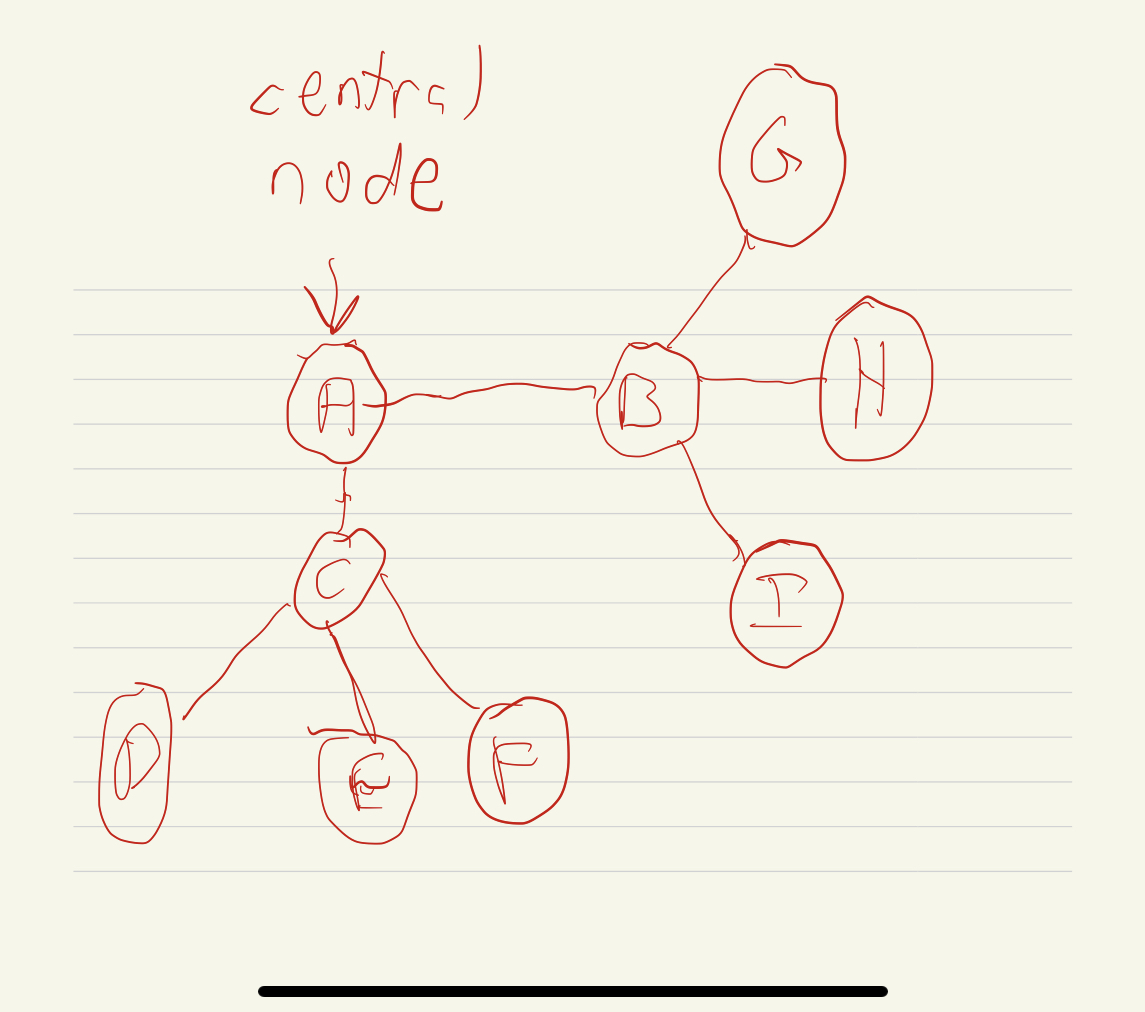
\includegraphics{graph1.jpg}

\textbf{2.)} \textbf{a.)} Is the directed graph in Figure 2 strongly
connected? If so, explain why; if not explain why not.

The graph is strongly connected as nodes that share a similar neighbor
also connect to each other in some fashion as if a node is being
directed or by a specific set of nodes it makes sense that eventually
those other nodes will form some kind of connection

\textbf{b.)} For the graph in Figure 2, if you think that it is not
connected what is the minimum number of directed edges that you would
need to add to make it strongly connected? If you think that it is
strongly connected what is the maximum number of edges that you can
remove such that the resulting graph is strongly connected

At most 1 directed edge can be removed for the graph to still represent
a strongly connected graph

\textbf{3.)} \textbf{a.)}Suppose you are interested in the social
network structure on a popular website named Y. Figure 3 shows such a
friendship network based on publicly available information from Y, where
solid lines represent strong ties and dashed lines represent weak ties.
Identify all bridges and local bridges in the network

The only bridge present is C-D as there are no other ways for both sides
to be connected

\textbf{b.)}Use the Strong Triadic Closure Property to find the
potential `hidden' friendships that aren't shown in Figure 3 but likely
exist in the real world.

When using the Strong Triadic Closure Property, a hidden friendship that
may be present that is not shown on the graph is D-G

\textbf{c.)} Add all hidden ties identified in (b) to the original
network (treat them as weak ties). Revisit the bridges and local bridges
you listed in (a): are they still bridges or local bridges?

There would still be a bridge present in the graph

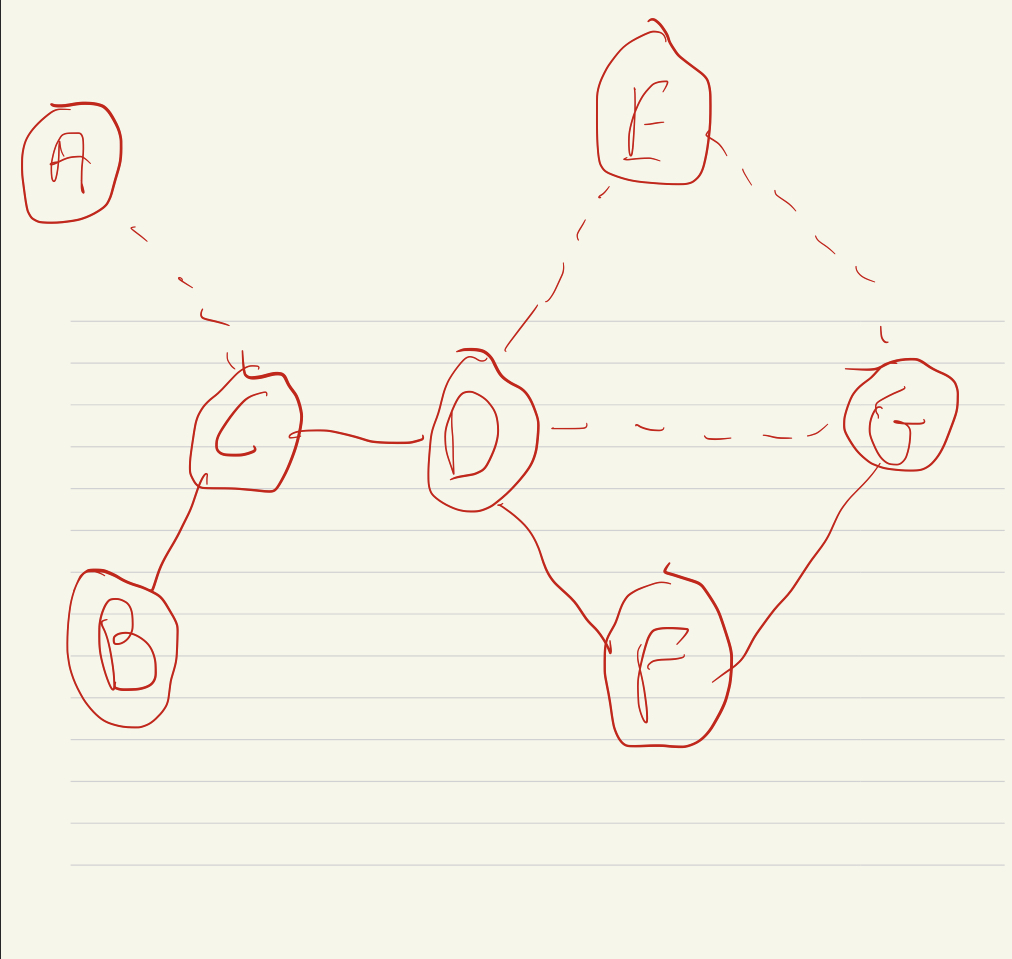
\includegraphics{graph2.jpg}

\textbf{4} \textbf{a.)}Construct a network of the five cities. Here's
how we'll decide to connect them: (i) If you can drive between two
cities in 150 miles or less, add a strong tie between them. (ii) If you
can't drive between two cities within 150 miles, but can do so in 200
miles or less, add a weak tie between them. You can travel on either a
direct route (a single road between cities) or an indirect route (a
combination of roads going through other cities). Once you've created
the network, write a list of all the strong ties and another list of all
the weak ties.

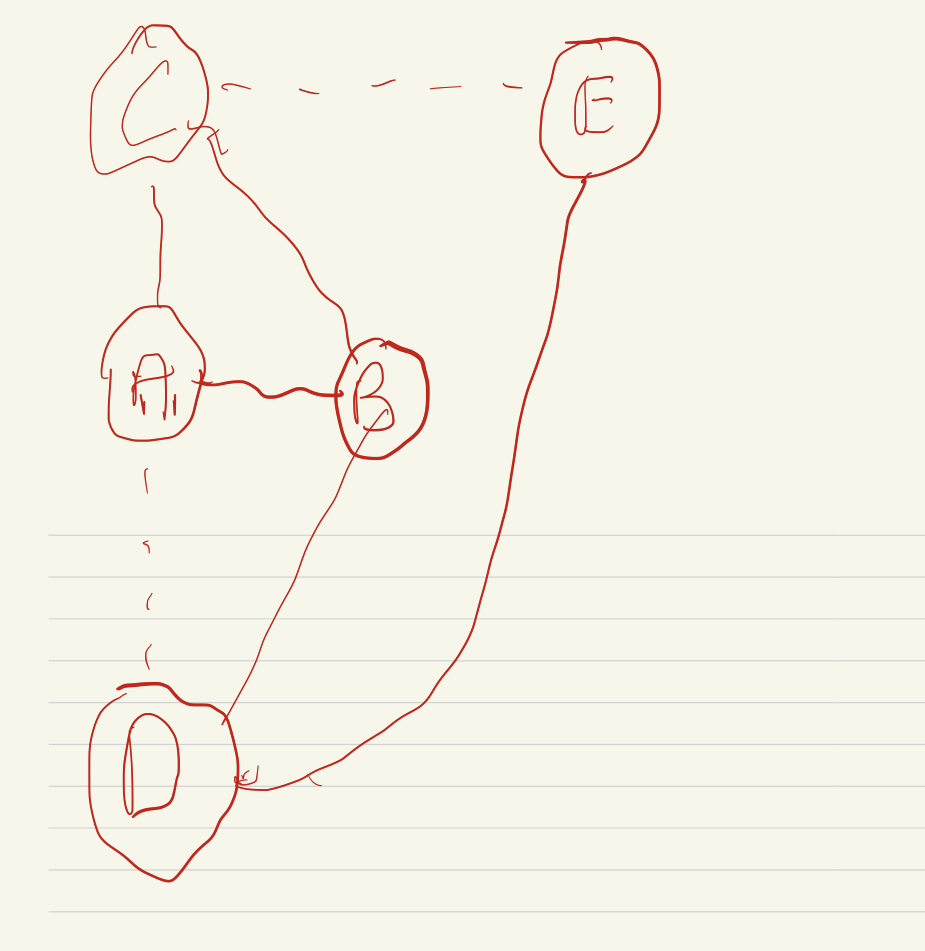
\includegraphics{graph3.jpg} The cities that satisfy the Strong Triadic
Closure Property are cities C,A,B as between these cities they have a
strong tie from one node. So it would make sense that if two nodes both
have a strong tie to one other node that those same nodes would also
have a strong tie between themselves. As for the cities that violate the
Strong Triadic Closure Property would be A,B,D as both A and D have a
strong tie to B so A and D should also have a strong tie between each
other but they instead have a weak tie.

\textbf{c.)} Can you change the `200 miles' threshold in our definition
of weak ties, so that the Strong Triadic Closure Property will always be
satisfied of all cities? Explain why

Yes this should be able to make it so that the Strong Triadic Closure
Property will always be satisfied of all cities, as this would make it
so that strong ties are formed between a set of 3 nodes where if the two
nodes have a strong leading to the other singular node then a strong tie
is also formed between them.

\textbf{5.)} \textbf{a.)}

What are the possible structures of a balanced complete graph with 4
nodes? For each possible scenario, draw an example and calculate the
number of negative edges in it.

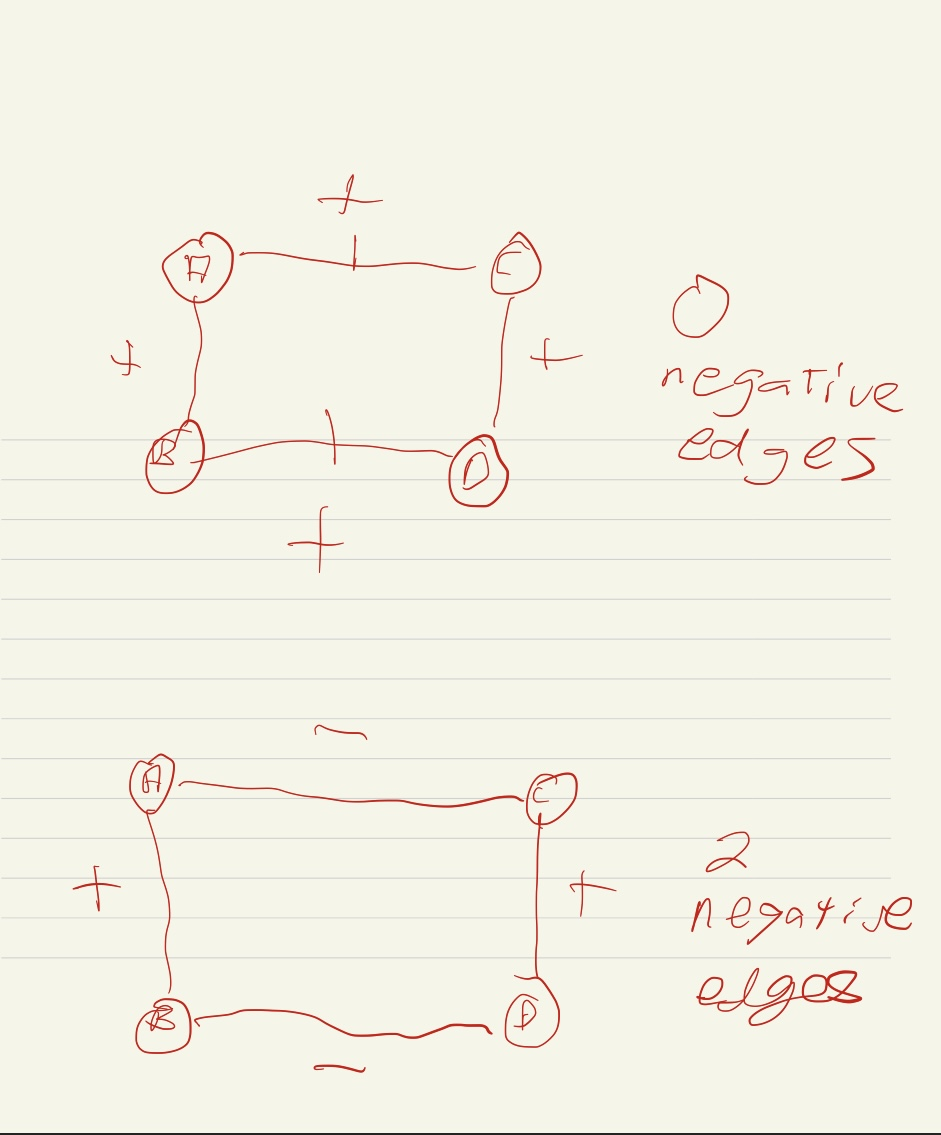
\includegraphics{graph4.jpg}

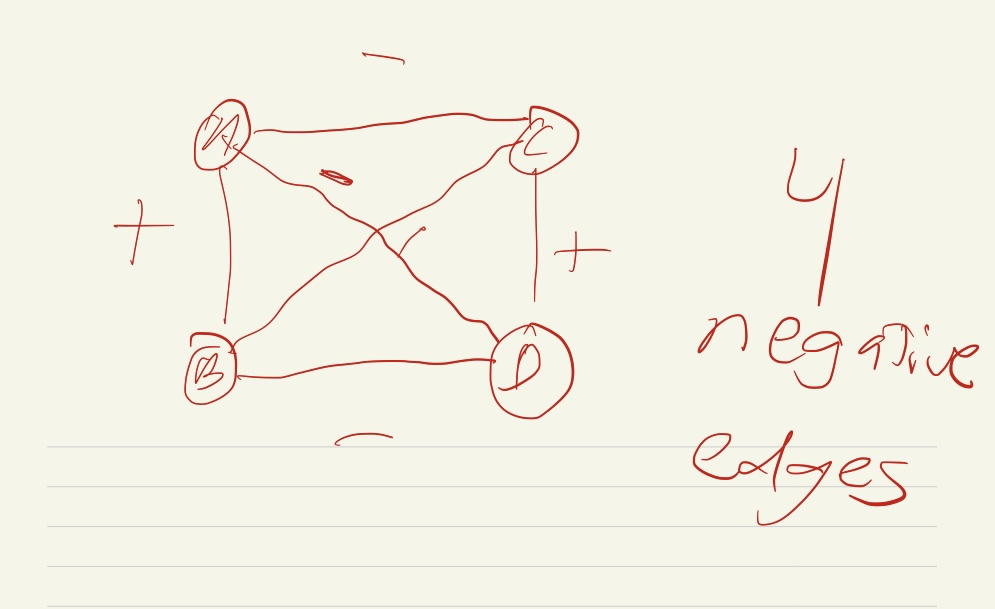
\includegraphics{graph5.jpg}

\textbf{b.)}

What are the possible structures of a balanced complete graph with 5
nodes? For each possible scenario, draw an example and calculate the
number of negative edges in it.

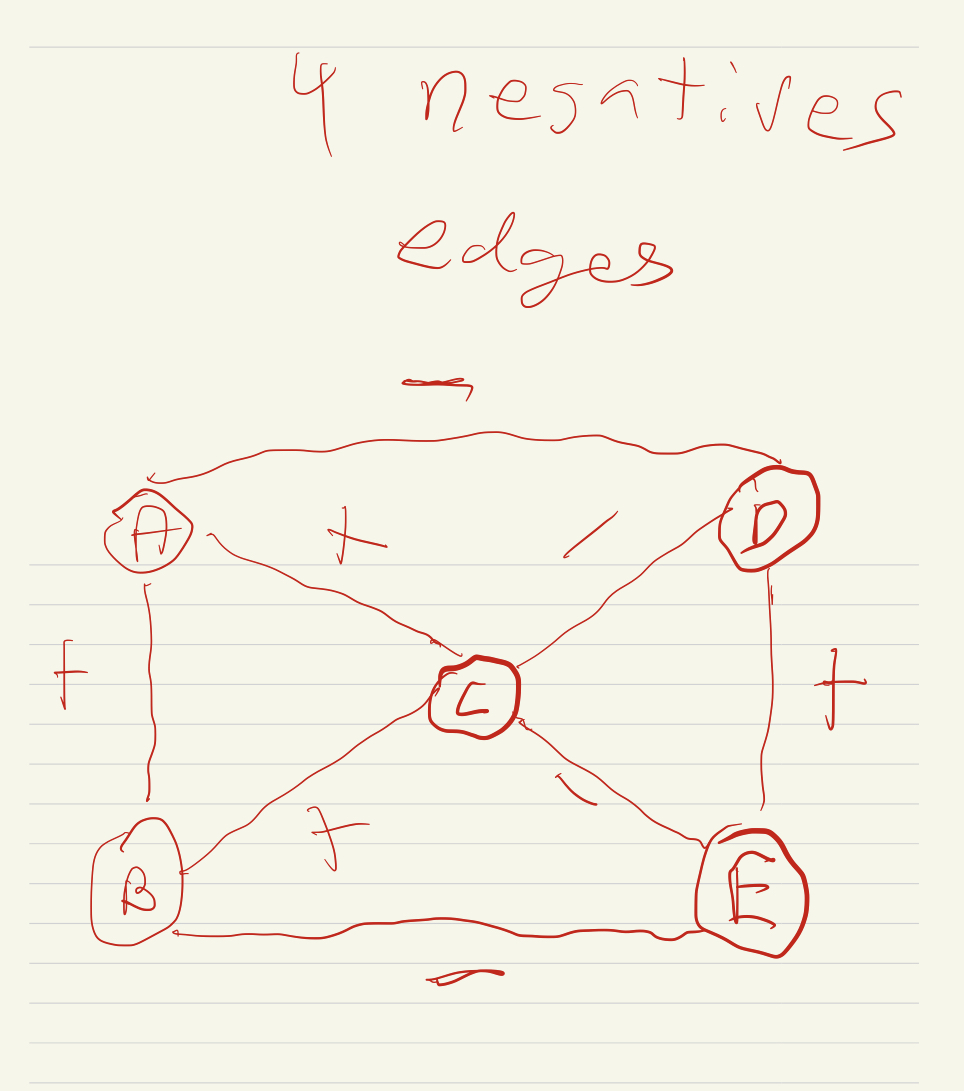
\includegraphics{graph6.jpg}

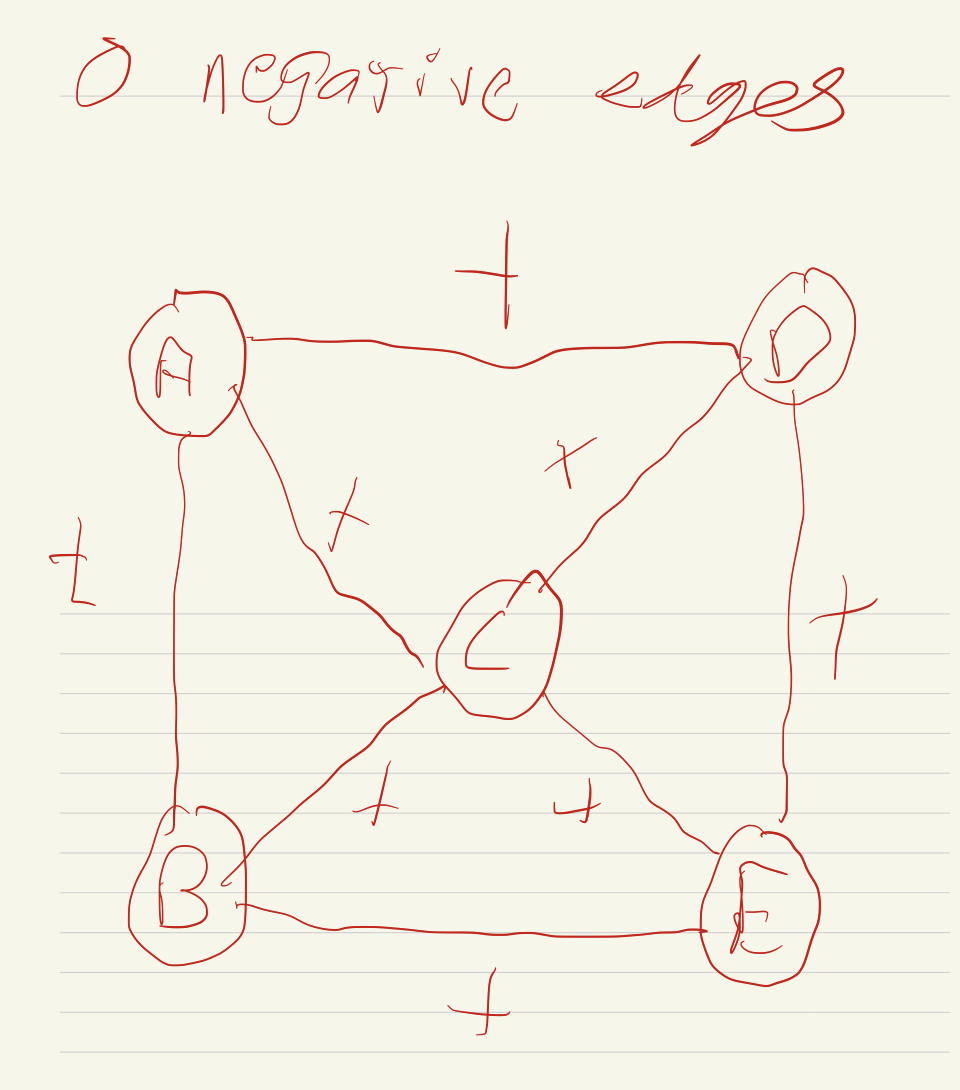
\includegraphics{graph7.jpg}

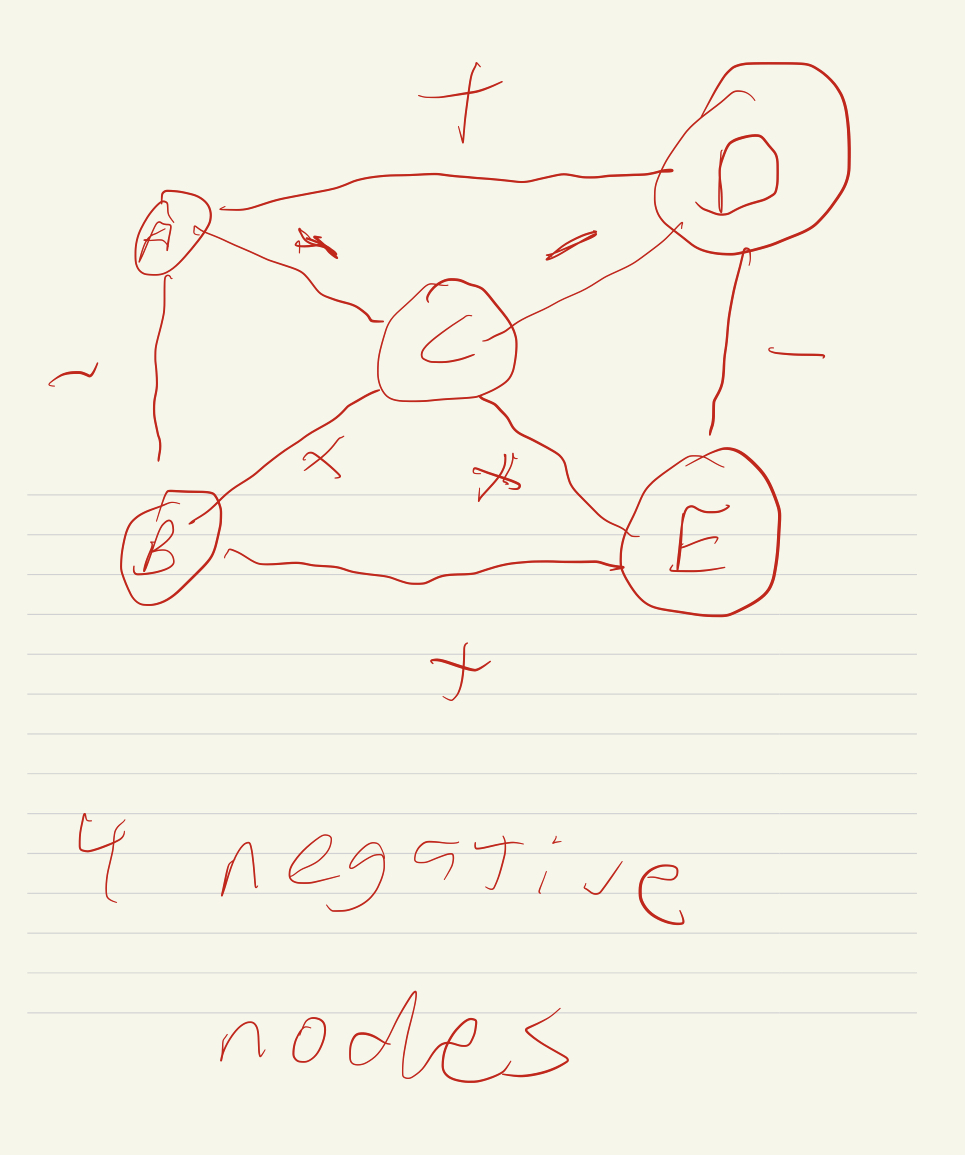
\includegraphics{graph8.jpg}

\textbf{c.)}

These exercises show how balanced theorem simplifies the counting of
different balanced structures. Indeed, if one takes a naive approach by
simply enumerating all possible signed complete graphs of 5 nodes (10
edges) and checking which of them are balanced, they will need to
examine 210 = 1, 024 different configurations! Now let's try to
generalize the results in (a) and (b): For an integer n ≥ 3, what are
the possible number of negative edges of a balanced complete graph with
n nodes?

\[\frac{n(n-1)}{n}\]

\end{document}
